\documentclass[conference]{IEEEtran}
\usepackage{cite}
\usepackage{amsmath,amssymb,amsfonts}
\usepackage{graphicx}
\usepackage[caption=false,font=footnotesize,labelfont=md,textfont=md]{subfig}
\usepackage{booktabs}
\usepackage{multirow}
\usepackage{balance}
\usepackage{verbatim}

\AtBeginDocument{%
  \setlength{\textfloatsep}{6pt plus 1pt minus 2pt}%
  \setlength{\dbltextfloatsep}{6pt plus 1pt minus 2pt}%
  \setlength{\floatsep}{6pt plus 1pt minus 2pt}%
  \setlength{\dblfloatsep}{6pt plus 1pt minus 2pt}%
  \setlength{\intextsep}{6pt plus 1pt minus 2pt}%
  \setlength{\abovecaptionskip}{4pt}%
}

\begin{document}

\title{Mining Egocentric Video with Sorter Speech for Plastic Classification}

\author{\IEEEauthorblockN{Yeonu Lee}
\IEEEauthorblockA{\textit{Mountain View High School} \\
\textit{High School Student} \\
Mountain View, CA, USA}
\and
\IEEEauthorblockN{Jamalia Sultana}
\IEEEauthorblockA{\textit{Dept.\ of Computer Science} \\
\textit{Stony Brook University}\\
Stony Brook, NY, USA}
\and
\IEEEauthorblockN{Zhaozheng Yin}
\IEEEauthorblockA{\textit{Dept.\ of Computer Science} \\
\textit{Stony Brook University}\\
Stony Brook, NY, USA}
}

\maketitle

\begin{abstract}
Sorting household plastics by hand remains standard practice at material recovery facilities (MRF), where it poses health issues for workers and problem of insufficient throughput to meet recycling demand. In order to address this problem, we mined Egowaste -- a dataset produced by material recovery facilities, where they paired visual and spoken records of the items workers handle. Specifically, it is a first-person dataset in which each clip captures a worker holding a plastic item while describing it aloud.
Our pipeline first masks the target object using a segmentation model, then selects the best candidate mask through a multi-stage scoring process: contrastive and supervised image models score each candidate crop, while a audio branch transcribes the sorter's speech using a LoRA-adapted Whisper model and matches the transcript against a phrase list to identify the spoken plastic category. Image-based and speech-based predictions are then combined via logistic regression to produce a final classification.
We evaluate the system at multiple stages, from mask overlap (intersection-over-union, IoU) to clip-level ``any frame correct'' accuracy. The best-performing vision-speech fusion setup achieves a group-level any-frame accuracy of 73.4\%, compared with 69.6\% for the strongest vision-only model.
We present stage-by-stage performance scores and confusion matrices for the mask, crop, and fusion configurations.
\end{abstract}

\begin{IEEEkeywords}
multimodal data mining, recycling and waste management, plastic classification, first-person vision, multimodal fusion
\end{IEEEkeywords}

\section{Introduction}
Recycling facilities generate material-wise waste sorting data, including video and the verbal descriptions sorters give as they work. Every item that passes a sorting station leaves a frame containing the image of the hand and the object, along with a spoken phrase that names the material or describes its characteristics, which is associated with a plastic class label. Mining these paired records means learning which appearances and which phrases go with each plastic type, which is exactly the decision a sorter makes during the waste sorting process. We therefore study how to mine this multimodal data to support fine-grained plastic sorting, a key step in waste management.
Automated waste-sorting shows up in many places: smart bins, conveyor belts in MRFs, outdoor litter cameras, underwater cleanup, and construction sites~\cite{gundupalli2017sorting,tamin2026review}.
Most existing work relies solely on RGB imagery, and while surveys report strong performance on clean lab sets, these models still struggle with overlapping, deformed, or visually similar plastic objects~\cite{thung2016trashnet,bashkirova2022zerowaste,yudin2024warp}.
Even setups that add sensing beyond RGB~\cite{friedrich2022sensor,luo2024mdcf} watch the stream from a fixed camera. None of them leverage the \emph{sorter's first-person viewpoint} or the short verbal phrases workers use to distinguish visually similar plastics.
A fully automatic line is also hard to run in practice. In several regions, MRF rules require a certified operator or supervisor on site, people checking the belt, and a plan for hazardous items~\cite{arkansas2024mrflicense,connecticut2024recycling,uk2022mrf,hse2024wasteprocessing}.
Thus, we suggest the vision being a \emph{helper for the sorter}, not a replacement.
We target MRF-style detailed plastic sorting while keeping the human sorter in the process.
Prior first-person datasets such as Ego4D~\cite{grauman2022ego4d} and IndEgo~\cite{chavan2025indego} (covering factory assembly, logistics, and spoken narration) already study egocentric hand-object interaction, but neither addresses MRF plastic categories or descriptive audio.
This setting is challenging as target objects are small, the hand occludes part of the object, and spoken phrases do not map one-to-one onto class labels. Table~\ref{tab:datasets} shows that existing collections do not capture this gap.

This paper makes four contributions:
\begin{itemize}
\item We evaluate end-to-end plastic sorting using the EgoWaste camera-1 subset, which contains \textbf{15 categories} and 463 video clips (3{,}538 frames).
\item We use \textbf{SAM3}~\cite{carion2025sam3} to cut out the object, then a \textbf{four-stage mask pick and rerank} so later crops are cleaner.
\item We combine \textbf{image models} (CLIP~\cite{radford2021learning}, SigLIP~\cite{zhai2023siglip}, EfficientNet-B0~\cite{tan2019efficientnet}) with \textbf{Whisper LoRA} transcription~\cite{radford2023whisper,hu2022lora} and \textbf{phrase matching} (Sentence Transformer MiniLM-L6-v2~\cite{reimers2019sentence}) on our common-phrase list, then join the two with logistic regression.
\item We report \textbf{stage-by-stage scores} from mask IoU to frame- and clip-level Top-1 accuracy, to assess the contributions of cropping, reranking, and speech at each stage of the pipeline.
\end{itemize}

Section~\ref{sec:related} reviews related work.
Section~\ref{sec:dataset} describes the dataset and task.
Section~\ref{sec:method} presents our pipeline.
Section~\ref{sec:experiments} reports experiments; Sections~\ref{sec:discussion}--\ref{sec:conclusion} discuss limits and next steps.

\section{Related Work}
\label{sec:related}

Public waste datasets differ in scene, view, audio, and label granularity (Table~\ref{tab:datasets}).
{TrashNet}~\cite{thung2016trashnet} is a common clean benchmark: one object on a plain background, with little overlap, motion, or factory lighting~\cite{tamin2026review}.
Light CNNs and mixed designs (EfficientNet, MobileNet, CustomNet) trained on TrashNet and merged household photos report $>$94--98\% accuracy on single, centered objects on Jetson or Raspberry Pi~\cite{thung2016trashnet,tamin2026review}.
{TACO}~\cite{proenca2020taco} labels outdoor litter under a 28-class tree with COCO-style instance masks, with class frequencies so uneven that papers often evaluate on merged groups.
Litter systems fine-tune Mask R-CNN or YOLO on TACO; underwater sets such as TrashCan and construction-waste detectors use different physics and class lists~\cite{proenca2020taco,tamin2026review}.
Plant-scale methods find flexible conveyor streams with YOLO detectors, hierarchical heads, or weakly labeled segmentation: ZeroWaste~\cite{bashkirova2022zerowaste} has semi- and weakly labeled variants, while WaRP~\cite{yudin2024warp} first finds five broad groups, then fine classes ($mAP_{50}$ 58.6\%), with overlapping flexible objects and masks trained from class labels only.
{UrbanWaste}~\cite{ma2025urbanwaste} watches household bins with before/after change detection (13{,}553 pairs).
Open-vocabulary segmentation (SAM3~\cite{carion2025sam3}, Grounding DINO~\cite{liu2023grounding}) and vision--language models (CLIP/SigLIP~\cite{radford2021learning,zhai2023siglip}) cut the cost of training a new detector for each plastic type when labeled data are scarce.
First-person fusion more often targets action recognition~\cite{grauman2022ego4d,radevski2023multimodal,alayrac2022flamingo} than material type.
Plants that cannot separate black film or mixed materials from RGB alone add NIR or induction sensing on a fixed camera~\cite{friedrich2022sensor,luo2024mdcf}.

\begin{table}[!t]
\caption{Comparison of waste datasets vs.\ EgoWaste camera-1 plastics (this work). Scenario tags follow~\cite{tamin2026review}.}
\label{tab:datasets}
\centering
\scriptsize
\setlength{\tabcolsep}{2pt}
\begin{tabular}{lcccc}
\toprule
Dataset & Scenario & View & Audio & Classes \\
\midrule
TrashNet & smart bin & studio & no & 6 \\
TACO & outdoor & in-the-wild & no & 60 \\
ZeroWaste & MRF belt & conveyor & no & 4 \\
WaRP & MRF belt & conveyor & no & 28 \\
UrbanWaste & smart bin & in-bin & no & 193 \\
EgoWaste & MRF (ours) & first-person & yes & 15 \\
\bottomrule
\end{tabular}
\end{table}

EgoWaste instead records pixel-level masks over 463 video clips and pairs each clip with the verbal phrases sorters use while working.
The extra modality we exploit is therefore the worker's own speech, not the impact sounds~\cite{luo2024mdcf,lu2022multimodal} or spectral readings earlier multimodal sorters rely on.

\section{Dataset and Task Formulation}
\label{sec:dataset}

%\subsection{EgoWaste Plastics Subset}
We use the EgoWaste camera-1 plastics shareable evaluation subset.
Each record has an RGB frame, a pixel-level true mask, a 15-way class label, a bounding box, and a matching video clip at the toss.
The evaluation split has \textbf{3{,}538} frames across \textbf{463} clips and \textbf{15} plastic types in a resin-based class list.
%\subsection{Taxonomy}
Classes include deposit and non-deposit bottles, numbered containers (\#1 clamshells, \#2 natural/colored, \#3--7), black plastic, garbage bags, and leftover groups such as unnumbered fragments.
See Table~\ref{tab:datasets} and Sec.~\ref{sec:related} for how this subset differs from prior waste collections.

%\subsection{Audio and Common Phrases}
In each video clip, workers say short phrases while they sort (for example, ``number one clamshell,'' ``five PP'').
We extract the soundtrack from each video clip and transcribe it.
We keep 104 unique \emph{common phrases} as training metadata and as a search index from Whisper text to class labels.
Fig.~\ref{fig:dataset} shows a frame--mask pair and class crops; spoken phrases are listed in the caption.

\begin{figure}[!t]
\centering
\subfloat[Frame + GT mask (GX010023, Black Plastic).]{%
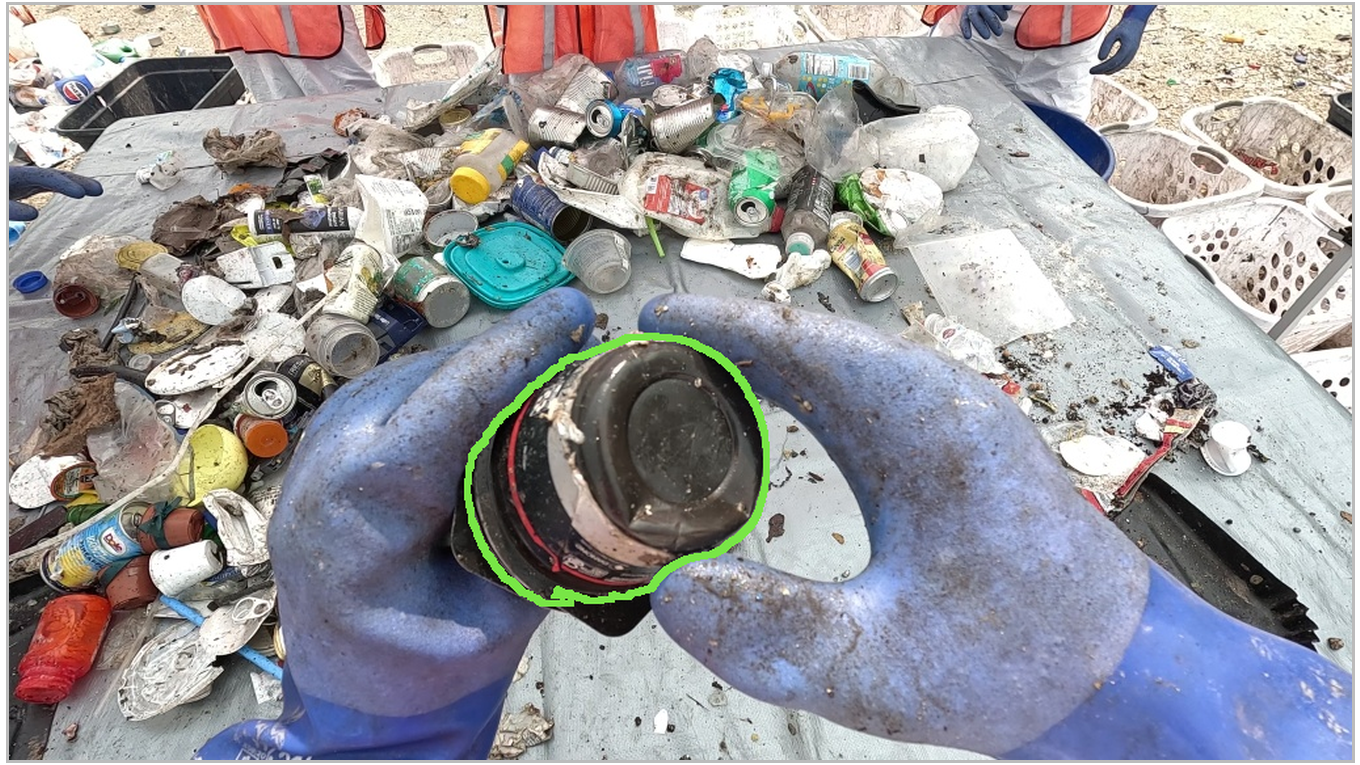
\includegraphics[width=\linewidth]{fig/dataset_sample_frame.png}%
\vspace{-0.25\baselineskip}%
\label{fig:dataset-a}}
\\
\subfloat[category\_name + GT masked crop.]{%
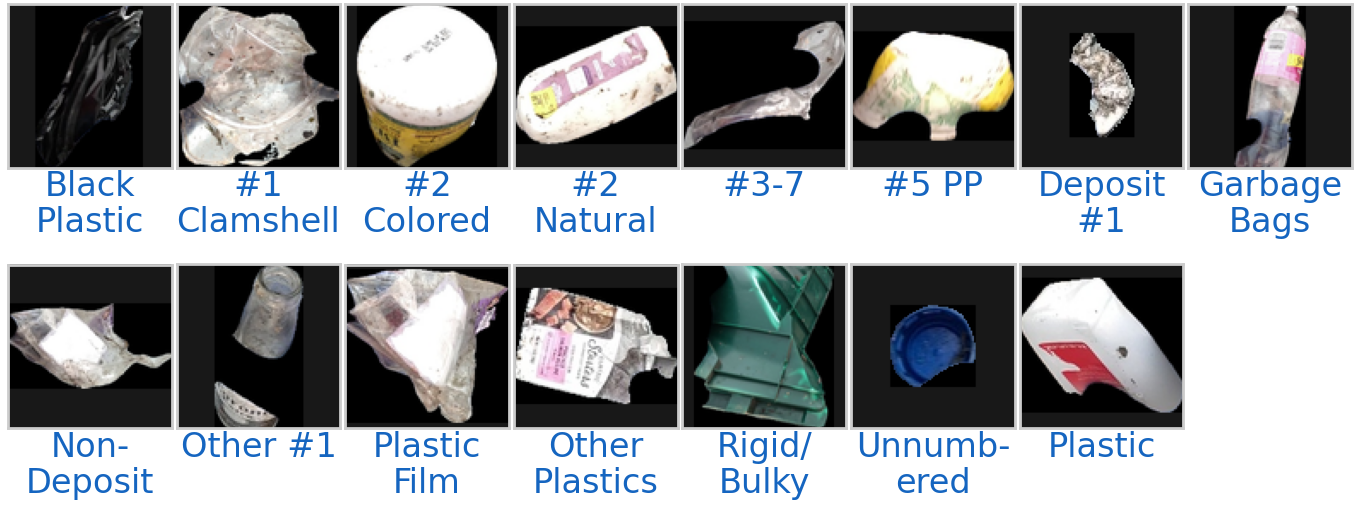
\includegraphics[width=\linewidth]{fig/dataset_sample_crops.png}%
\vspace{-0.5\baselineskip}%
\label{fig:dataset-b}}
\caption{Dataset samples. Spoken common phrases in (b), left to right, top to bottom: ``unnumbered black plastic,'' ``one clamshell,'' ``two colors,'' ``natural,'' ``three to seven,'' ``five,'' ``one deposit,'' ``non-deposit garbage bag,'' ``other non-deposit,'' ``non-deposit one,'' ``film plastic,'' ``do we have other plastic?,'' ``bulky rigid,'' ``unnumbered,'' ``other plastic.''}
\label{fig:dataset}
\end{figure}

\section{Method}
\label{sec:method}

\begin{figure*}[!t]
\centering
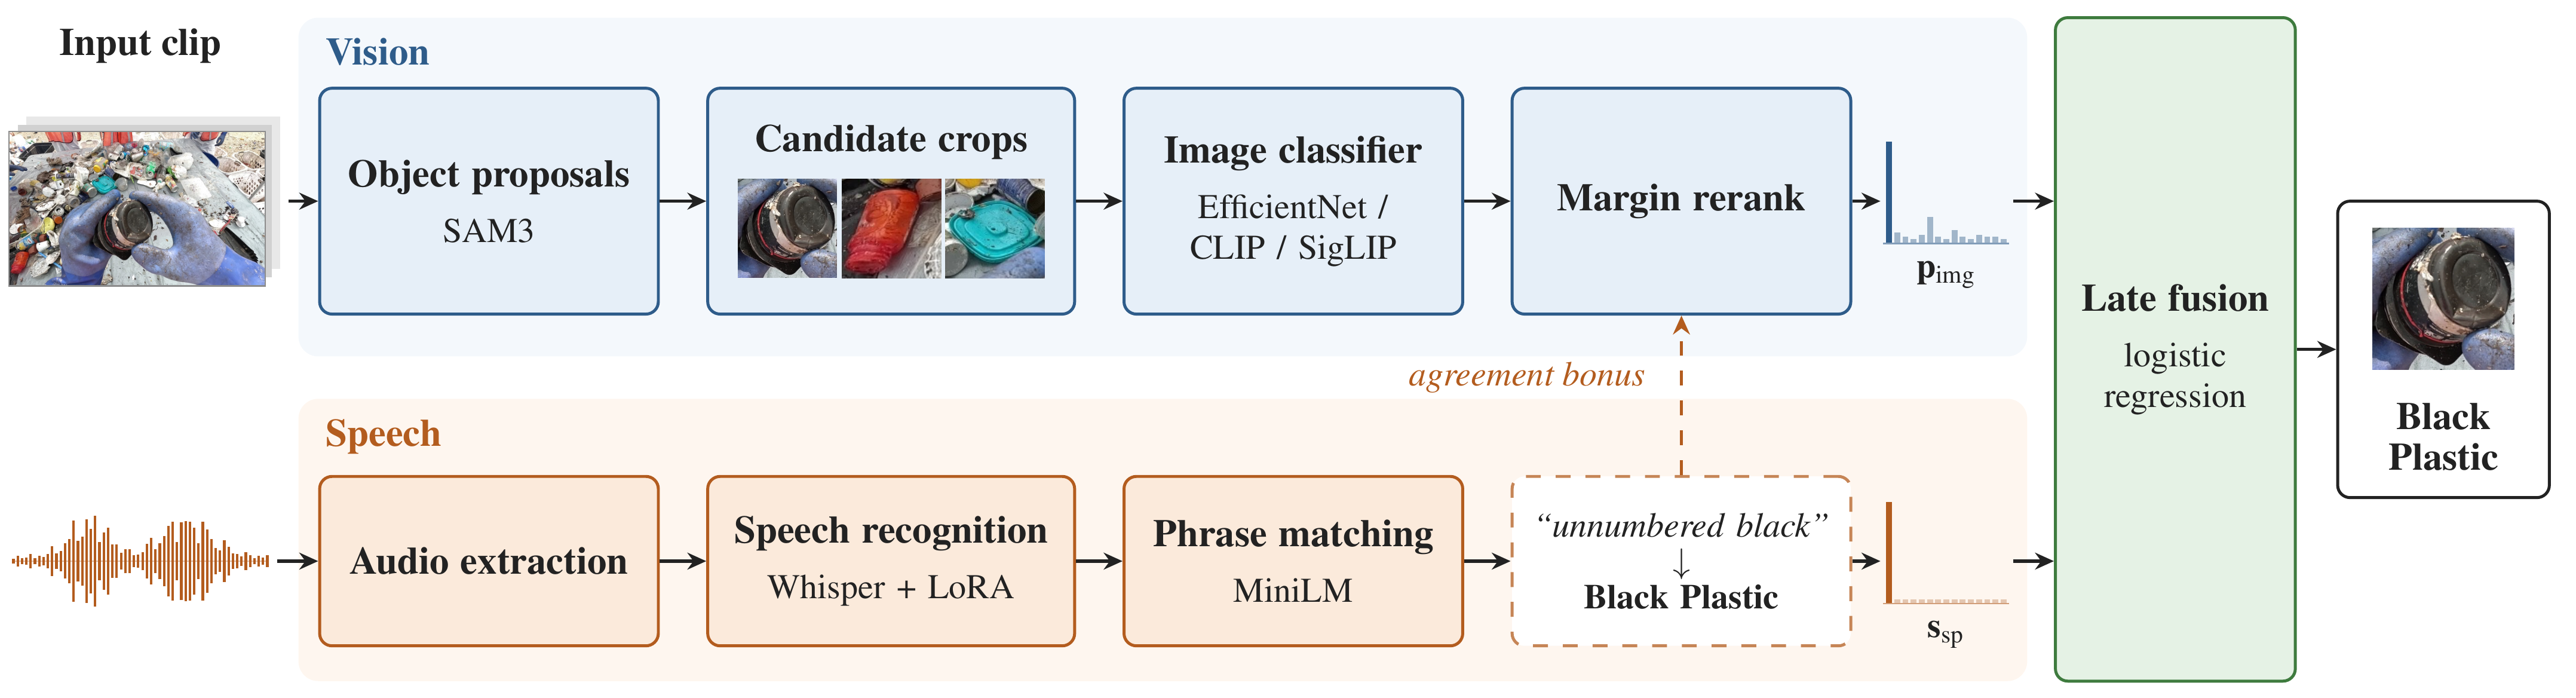
\includegraphics[width=\textwidth]{fig/fig2_compare_mod.png}
\caption{System overview for one input clip. \textbf{Vision branch} (per frame): SAM3 object proposals $\rightarrow$ candidate crops $\rightarrow$ image classifier (EfficientNet-B0, CLIP, or SigLIP) $\rightarrow$ margin rerank by the gap between the top two class scores, yielding the 15-D score vector $\mathbf{p}_\mathrm{img}$. \textbf{Speech branch} (per clip): audio extraction $\rightarrow$ Whisper+LoRA speech recognition $\rightarrow$ MiniLM phrase matching, which maps the spoken phrase (here ``unnumbered black'') to a class and yields the one-hot vector $\mathbf{s}_\mathrm{sp}$. The dashed \emph{agreement bonus} feeds that spoken class back into margin rerank. Late fusion logistic regression joins $\mathbf{p}_\mathrm{img}$ and $\mathbf{s}_\mathrm{sp}$ into the final class (here Black Plastic).}
\label{fig:pipeline}
\end{figure*}

Fig.~\ref{fig:pipeline} shows the pipeline.
On each frame, SAM3~\cite{carion2025sam3} proposes object masks, we classify the crops, and we apply margin rerank by the gap between the top two class scores.
On each clip we extract the soundtrack, transcribe it with Whisper+LoRA, and map it to a class with MiniLM phrase matching and text rules; an agreement bonus from speech to vision can boost a matching crop, and late fusion logistic regression joins the two branches.

\subsection{Problem Setup}
We score at the \textbf{frame level} (each labeled frame) and the \textbf{group level} (463 video clips).
A clip is correct under an \emph{any-frame any-bbox} rule: if any frame's predicted class matches the clip label, using the best mask for that setting, the clip counts.
The main end-to-end number is \textbf{final-probability Top-1} after we drop failed masks and calibrate probabilities. We also report mask IoU versus the true outline and segment-level class Top-1 accuracy in Table~\ref{tab:pipeline}.

\subsection{Detection and Mask Selection}
\textbf{Hand-crop detection} asks SAM3~\cite{carion2025sam3} only inside a hand-guided region and keeps the in-hand mask that sits most inside that region, or the largest box if that fails.
\textbf{Full-image detection} runs Top-5 plastic segmentation over the whole frame.
Mask IoU rises from 8.3\% (hand crop) to 19.8\% (full image). Tight hand crops often cut off the object.

Phases 1--4 then clean up the mask list: Ph.1 classifies crops from the two detection strategies; Ph.2 adds candidates, optional masked crops, and padded boxes (the main accuracy jump is picking a better mask); Ph.3 uses Top-5 pools that mix in-hand, full-image, and score-ranked masks; Ph.4 reranks by score margin and, at clip level, gives extra credit when Whisper matches vision.
For each frame we keep up to five mask candidates. We score them by how much they sit in the hand region, how they overlap SAM3~\cite{carion2025sam3} confidence, and simple edge/contact checks from the segment code.
Reranking keeps the candidate with the largest gap between the top two classifier scores, and may add a bonus when Whisper agrees with vision.
Masked crops black out pixels outside the mask before resize. Box crops with 15\% padding are a lighter backup when the mask edge is shaky.

\subsection{Vision Classifiers}
We train all image models on the same train/validation split, sampling so each class appears in proportion to the data.
CLIP and SigLIP linear probes train one layer on frozen patch features. LoRA adapters sit on attention projections with rank 8.
EfficientNet-B0 is fine-tuned end-to-end with standard augmentations (random resized crop, color jitter).
We pick checkpoints on validation final-probability Top-1 and run them once on held-out evaluation frames.
Crops (box by default; masked crops when we turn that piece off) go into:
\begin{itemize}
\item \textbf{Zero-shot:} CLIP and SigLIP, each with 15-class prompts.
\item \textbf{Linear probe \& LoRA} for CLIP ViT-B/32 and SigLIP.
\item \textbf{EfficientNet-B0:} supervised fine-tuning on training folds.
\end{itemize}
Classifiers output 15-way class scores that sum to 1.

\subsection{Audio Pipeline}
We extract audio from each video clip and transcribe it with \textbf{Whisper large-v2 + LoRA} (rank 8, $\alpha{=}32$ on query/value projections).
Transcripts map to classes in two ways: (i)~\textbf{meaning-based search}: embed the transcript and all common phrases with a MiniLM sentence encoder~\cite{reimers2019sentence}, take the closest phrase, then read its class; (ii)~\textbf{simple text rules} for common speech-to-text errors (for example, ``non deposit garbage bag'' $\rightarrow$ Non-Deposit).
We cache per-clip phrase maps for fusion training and test.

\subsection{Late Fusion and Metrics}
At the end we join the 15-D image scores with a 15-D one-hot speech class (zeros if unknown) and train \textbf{logistic regression} on the training split.
Two fusion variants pair CLIP or EfficientNet images with Whisper text (\emph{Fusion}, \emph{Fusion-EN}).
Metrics: mask IoU, segment class Top-1, frame/group final-probability Top-1, and how often the pipeline succeeds.

\section{Experiments and Results}
\label{sec:experiments}

All experiments run in PyTorch on NVIDIA GPUs. SAM3~\cite{carion2025sam3} produces hand-crop and full-image detections; exported masks feed mask selection and reranking in Table~\ref{tab:pipeline}.
Whisper LoRA uses learning rate $10^{-4}$, batch 8, and 3 epochs on toss-audio transcripts. Phrase search uses 384-D MiniLM embeddings; cosine similarity picks the Top-1 common phrase, then we look up the class.
Fusion logistic regression trains on joined 30-D training-split features. Evaluation rolls per-frame JSON into clip scores by majority vote and any-frame any-bbox.
A fixed scoring script compares five classifier families---CLIP and SigLIP linear probes, EfficientNet-B0, Fusion (CLIP+Whisper), and Fusion-EN (EfficientNet+Whisper)---at the representative settings of each phase in Table~\ref{tab:pipeline}.
On the final pipeline, EfficientNet segment class Top-1 is 61.2\% on 3{,}538 frames; final-probability Top-1 (67.8\%) uses the same mask filter as our reported pipeline.

\subsection{Phase-Wise End-to-End Accuracy}

\begin{table}[!t]
\caption{End-to-end final-probability Top-1 (\%) by pipeline stage. Det.: mask IoU. Group row: any-frame any-bbox over 463 clips with speech-aligned reranking.}
\label{tab:pipeline}
\centering
\resizebox{\columnwidth}{!}{
\small
\begin{tabular}{lccccc}
\toprule
Stage & CLIP & SigLIP & EffNet & Fusion & Fus.-EN \\
\midrule
\multicolumn{6}{l}{\textit{Detection (mask IoU only)}} \\
\quad Hand crop & \multicolumn{5}{c}{Mask IoU = 8.3} \\
\quad Full image & \multicolumn{5}{c}{Mask IoU = 19.8} \\
\midrule
Ph.1 Backbone & 15.7 & 14.4 & 21.8 & 19.7 & 22.0 \\
Ph.2 Mask select & 38.8 & 36.9 & 49.9 & 46.4 & 51.3 \\
Ph.3 Rerank pool & 40.8 & 39.8 & 57.4 & 49.8 & 58.7 \\
Ph.4 Margin rerank & 39.9 & 39.0 & 57.5 & 49.7 & 58.6 \\
Group (speech-align.) & 56.8 & 55.1 & 69.6 & 69.1 & \textbf{73.4} \\
\bottomrule
\end{tabular}}
\end{table}

Table~\ref{tab:pipeline} lists frame-level final-probability Top-1 (\%) by stage and a group row over 463 clips (any-frame any-bbox).
Raising mask IoU from 8.3\% (hand crop) to 19.8\% (full-image detection) helps, but the large accuracy jump is at Phase 2, when we choose better crops. Early errors come more from a bad crop than from raw IoU alone.
EfficientNet and Fusion-EN keep climbing in Phase 3. CLIP and SigLIP linear probes stay below 41\% on frames even after reranking.
Phase 4 barely changes frame scores, but it lets us add a Whisper-agreement bonus at clip-level evaluation.
On clips, Fusion-EN reaches \textbf{73.4\%}, ahead of EfficientNet (69.6\%) and Fusion-CLIP (69.1\%).

\subsection{Speech Ablations}
Table~\ref{tab:speech} scores the speech branch alone on the same 463 clips (no mask gate).
GT for WER is the clip's common phrase.
Base Whisper often inserts extra words, so mean WER can exceed 100\%; LoRA cuts it from 142.2\% to 33.3\%.
MiniLM (semantic) beats text rules at both settings (67.0\% vs.\ 61.3\% without LoRA; 81.9\% vs.\ 79.1\% with LoRA).
Speech-only Top-1 (LoRA+semantic, 81.9\%) is higher than Fusion-EN (73.4\%) because the end-to-end score still requires a valid mask; fusion helps most when vision is already close and the phrase names deposit vs.\ non-deposit.

\begin{table}[!t]
\caption{Speech-only clip accuracy (\%) and WER vs.\ the common-phrase transcript (463 clips).}
\label{tab:speech}
\centering
\scriptsize
\begin{tabular}{lccc}
\toprule
ASR & WER & Rules acc. & Semantic acc. \\
\midrule
Whisper (no LoRA) & 142.2 & 61.3 & 67.0 \\
Whisper + LoRA & \textbf{33.3} & 79.1 & \textbf{81.9} \\
\bottomrule
\end{tabular}
\end{table}

\begin{figure*}[!t]
\centering
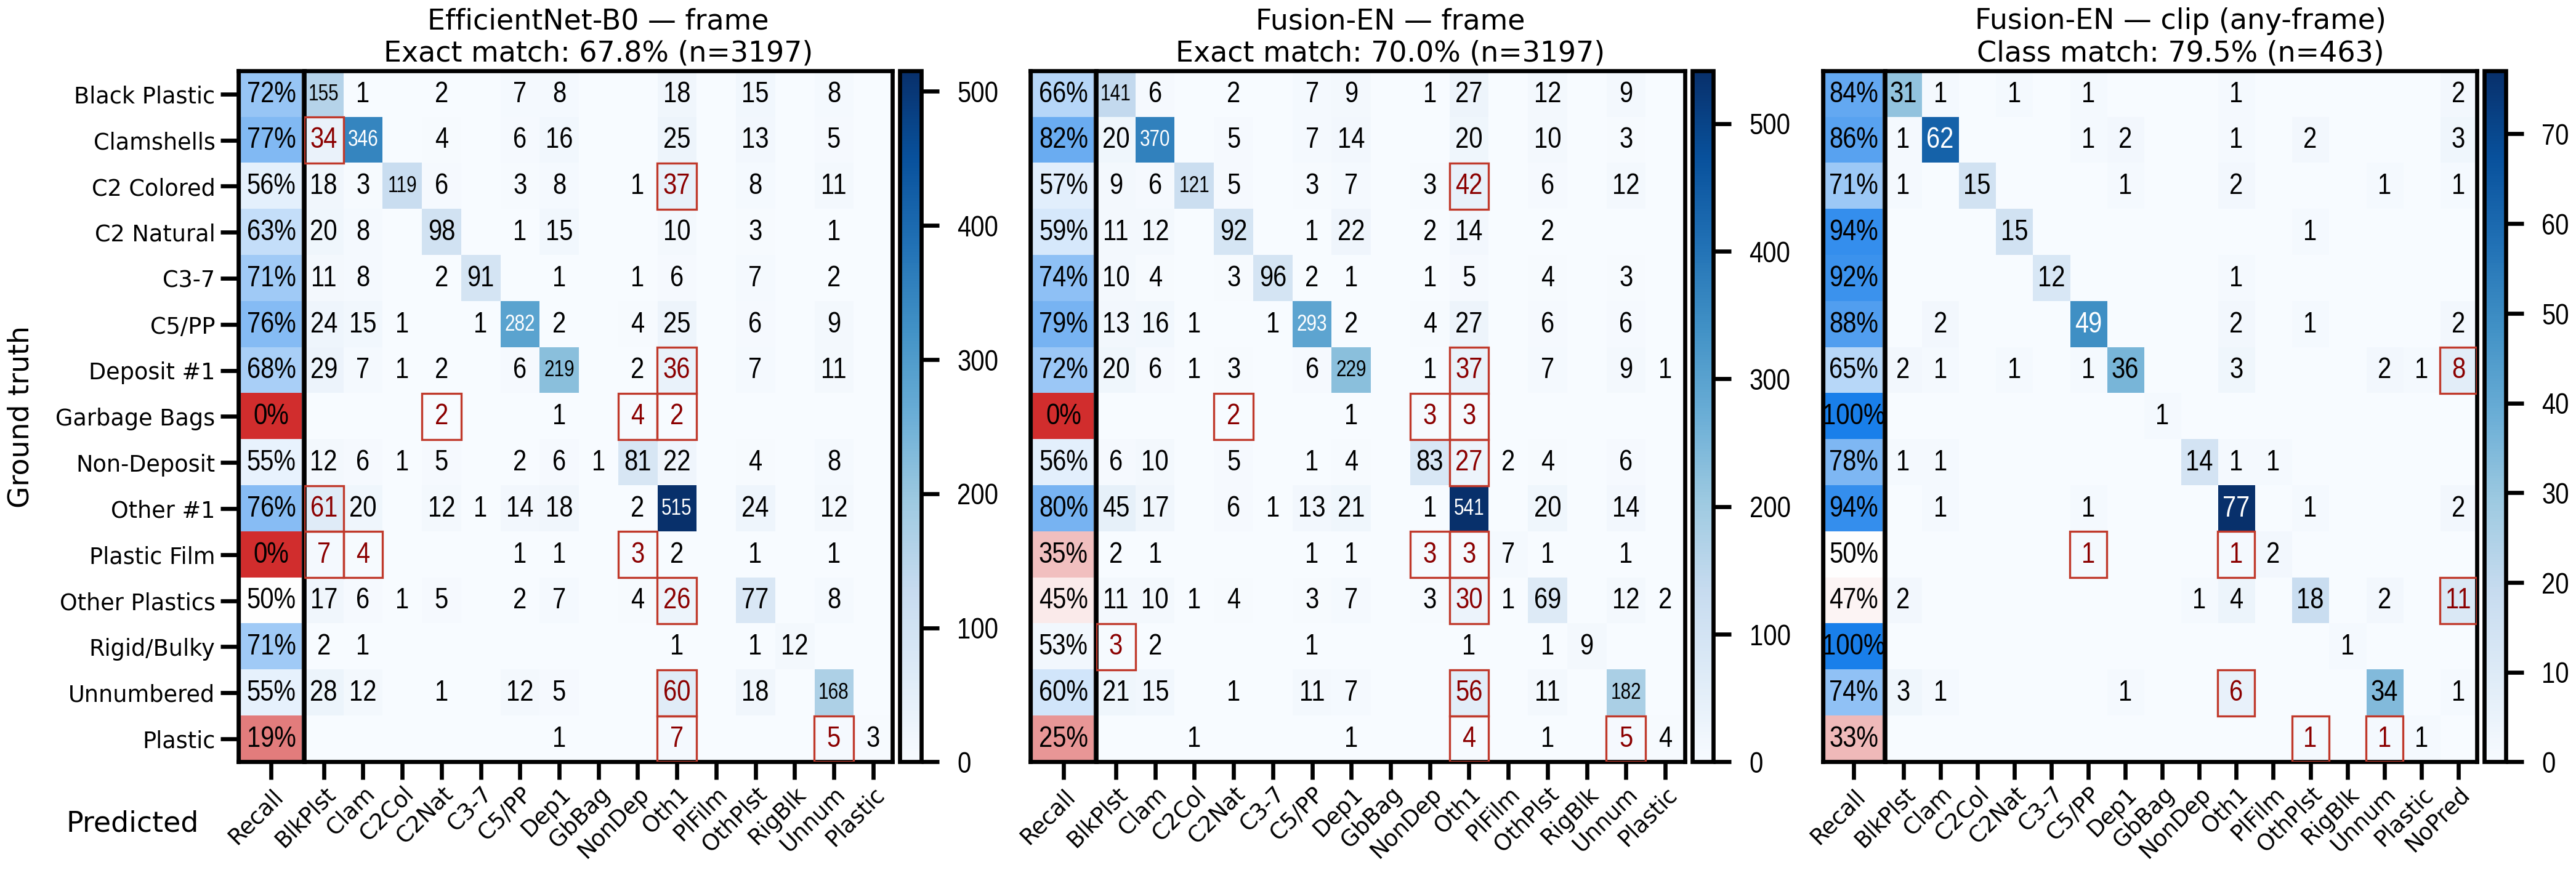
\includegraphics[width=\textwidth]{fig/confusion_matrix_best_models_row.png}
\vspace{-1\baselineskip}
\caption{Confusion matrices for the final pipeline: EfficientNet-B0 and Fusion-EN at the frame level, and Fusion-EN over the 463 clips under the any-frame rule used in Table~\ref{tab:pipeline} (clip correct when any frame predicts the labeled class; missed clips are charted with their majority prediction). The leftmost column of each panel is per-class recall; red boxes mark confusions above 7\% of a row (15\% for rows with few samples).}
\label{fig:confusion}
\end{figure*}

\subsection{Best Models and Confusion Analysis}
On \textbf{frame-level} evaluation with the final pipeline, EfficientNet reaches 67.8\% and Fusion-EN 70.0\% final-probability Top-1 (3{,}197 frames with a working mask).
Under the \textbf{any-frame} clip rule, Fusion-EN names the right class in 79.5\% of the 463 clips before the mask gate, which the gate turns into the 73.4\% reported in Table~\ref{tab:pipeline}.
Fig.~\ref{fig:confusion} compares the two frame-level matrices with the any-frame clip matrix of Fusion-EN.

\textbf{Uneven class counts.}
The class distribution is highly imbalanced. \emph{Other \#1 Bottles} is 732/3{,}538 instances (20.7\%). Garbage Bags (9), Other Plastic Film (22), Plastic (20), and Other Rigid/Bulky Plastics (18) are each $<$1\% of labels.
With even sampling, the head prefers the common class. On frames, 19.7\% of Unnumbered containers, 17.3\% of \#2 Colored, and 17.0\% of Other Plastics are called Other \#1, even when the true resin is different.
Rare classes have zero recall for Garbage Bags and Film with EfficientNet and stay below 35\% for generic Plastic and Film even with Fusion-EN.

\textbf{Mix-ups among similar classes.}
Five common misclassification groups show up:
(1)~\textbf{\#1 bottle family}---Deposit \#1, \#1 Clamshells, and Other \#1 share similar round PET geometries;
(2)~\textbf{\#2 HDPE family}---\#2 Natural vs.\ \#2 Colored differ primarily in color, making them difficult to distinguish visually;
(3)~\textbf{Black/dark cluster}---Black Plastic takes errors from Deposit \#1, Clamshells, and Unnumbered pieces when the hand covers the object;
(4)~\textbf{Catch-all vs.\ specific}---Unnumbered fragments and Other Plastics leak into numbered container classes;
(5)~\textbf{Rare/ambiguous materials}---Film, garbage bags, and generic Plastic have no rigid shape.
Speech fusion improves performance when the associated verbal phrases are lexically distinct (e.g., deposit vs.\ non-deposit). However, its benefit is limited in cases where the segmentation mask fails to capture the target object, or where automatic speech recognition produces a truncated or corrupted transcript.


\textbf{Fixing the uneven classes.}
Given that the Other-\#1 hub accounts for a substantial proportion of classification errors, we retrained the image model with \emph{inverse-frequency class weights}, where errors on rare classes would result in a higher penalty than errors on common classes.
This cut the frame-level false-positive rate into Other \#1 from 16.3\% to 11.7\% and raised macro-F1 by 1.2\%, while clip accuracy stayed about the same (73.4\% $\rightarrow$ 72.8\%).
Unnumbered container recall showed the largest improvement (+12.8\%), consistent with expectations, as these items were the primary source of incorrect Other-\#1 predictions.
We additionally evaluated oversampling of rare-class images across training epochs; however, this approach did not yield improvement. As rare classes contain only 9--22 unique crops, oversampling caused the model to memorize specific instances rather than generalize to the underlying class.
These results indicate that loss rebalancing helps visually similar container classes, whereas rare materials need additional data.

\subsection{Qualitative Examples}
Successes usually have a centered mask, a medium-size object, and a spoken phrase that sits in our list; failures often stack a missed hand crop, a chopped transcript (``5,'' for \#5 PP), or clear vs.\ colored \#2 bottles in bad light.
Late fusion recovers several deposit vs.\ non-deposit clips that EfficientNet misses when the bottle label is covered, but when both the mask and speech-to-text fail, no fusion model beats chance---later gains likely need better masks and audio together, not only a rerank after the fact.

\section{Discussion}
\label{sec:discussion}
Vision-speech fusion provides the greatest benefit when mask quality is already high: Fusion-EN outperforms EfficientNet by 0.2\% at Phase 1, but by 3.8\% at clip-level evaluation, where audio tells deposit status and resin hints apart.
Whisper plus phrase search fails when the transcript is empty or matches the wrong phrase; text-based rules mitigate but do not eliminate these failure cases.
Class weighting is an inexpensive fix for uneven class counts: it trims the Other-\#1 false-positive hub and lifts macro-F1 without extra data, but it does not help the rarest materials, and oversampling likewise fails without more examples.
Limitations include a plastics-only 15-class taxonomy, hand-crop sensitivity, scarce rare-class data, and no glove-versus-object mask in the final pipeline. Separate \#1/\#2 heads, more data, and stronger detectors would likely help.

\section{Conclusion}
\label{sec:conclusion}
We built a vision-plus-speech pipeline for detailed plastic sorting on EgoWaste. It uses SAM3~\cite{carion2025sam3} masks, four-stage reranking, image classifiers, Whisper LoRA transcripts, phrase matching, and logistic regression at the end.
Stage-by-stage scores show that masks and candidate reranking drive early gains, while speech adds a steady lift at the clip level (73.4\% group any-frame accuracy for Fusion-EN).

\balance
\bibliographystyle{IEEEtran}
\bibliography{refs}

\begin{comment}
\newpage
\section*{Supplementary Material}
\addcontentsline{toc}{section}{Supplementary Material}
\setcounter{section}{0}
\renewcommand{\thesection}{S\arabic{section}}

\section{Class-Balancing Experiments}
\label{app:balance}

The confusion analysis (Sec.~V-E) shows two limits on detailed accuracy: \emph{(i)} the dominant \emph{Other \#1 Bottles} class (732/3{,}538 training instances, 20.7\% of labels) soaks up false positives from visually similar containers, and \emph{(ii)} Garbage Bags (9), Other Plastic Film (22), Plastic (20), and Other Rigid/Bulky Plastics (18) have so few examples that they reach only 0--44\% group recall with the current even-sampling EfficientNet-B0 trainer.
We ran three balancing strategies on the same final pipeline and the same held-out 463-clip split. The numbers below are \textbf{measured}, from 5-epoch image fine-tuning with the late-fusion head left unchanged.

\subsection{Experimental Protocol}
All variants keep SAM3 crops from the best clip-level setting, the same train/validation clip split, and the same late-fusion training. Only the image-model loss and the sampler change.
\textbf{A0 (baseline):} current even cross-entropy (pipeline table: Fusion-EN group 73.4\%).
\textbf{A1 (inverse-frequency weights):} per-class loss weight $w_c = \bar{N}/N_c$, capped at $w_{\max}=10$ so the 9-sample Garbage Bags class does not blow up the gradient.
\textbf{A2 (epoch oversampling):} each training epoch resamples so every class appears at least $K{=}80$ crops (with replacement if $N_c{<}80$), keeping clip boundaries.
\textbf{A3 (A1 + A2 + focal loss):} $\mathcal{L}_{\text{focal}} = -\alpha_c (1-p_t)^\gamma \log p_t$ with $\gamma{=}2$ and $\alpha_c$ from A1.

Metrics: group final-probability Top-1 (mask success $\times$ class-given-mask, as in Table~\ref{tab:pipeline}), per-class recall on the rare types, macro-F1, and the false-positive rate \emph{into} Other \#1 from Unnumbered, \#2 Colored, and Other Plastics.
Group scoring matches Table~\ref{tab:pipeline}: the mask filter comes from the main pipeline run, and only the class prediction is re-run with each variant's checkpoint.

\subsection{Measured Results (463-clip group evaluation)}
Table~\ref{tab:balance_meas} compares each variant with A0 on the same group score as Table~\ref{tab:pipeline} (463 clips, 1{,}640 scored frames, any-frame any-bbox).
No variant met our pre-set target of $\geq$2~pp on group Top-1. Still, \textbf{A1 (reweight)} is the useful result: it dropped the frame-level false-positive rate into Other \#1 from 16.3\% to 11.7\% ($-$4.6~pp, a 28\% relative drop), raised macro-F1 by 1.2~pp, and improved Unnumbered recall by 12.8~pp, at a cost of only 0.6~pp in group Top-1.
A2 and A3 cut Other-\#1 false positives by a similar amount, but A2 lowered macro-F1 and A3 added complexity without beating A1 on rare-class recall.

\begin{table}[!t]
\caption{Measured group Top-1 and rare-class recall after class balancing (Fusion-EN, final pipeline, 463 clips). Group matches Table~\ref{tab:pipeline} (mask success $\times$ class-given-mask, \%); Macro-F1 and Other-\#1 FP are changes vs.\ A0; Film and Garbage Bags are group recall (\%).}
\label{tab:balance_meas}
\centering
\scriptsize
\setlength{\tabcolsep}{3pt}
\resizebox{\columnwidth}{!}{%
\begin{tabular}{lccccc}
\toprule
Variant & Group & Macro-F1 & O\#1 FP & Film & Bags \\
\midrule
A0 baseline & 73.4 & -- & -- & 50 & 50 \\
A1 reweight & 72.8 & +1.2 & $-$4.6 & 33 & 50 \\
A2 oversample & 72.6 & $-$2.2 & $-$5.8 & 17 & 50 \\
A3 combined & 72.1 & +0.4 & $-$5.8 & 17 & 50 \\
\bottomrule
\end{tabular}}
\end{table}

\subsection{Mix-ups Targeted by Balancing}
Reweighting goes straight at the main failure mode from Sec.~V-E: false positives \emph{into} Other \#1 from visually similar bottles and containers (Unnumbered, \#2 Colored, Other Plastics), mix-up group~(1).
A1 shrank that hub while raising Unnumbered recall by 12.8~pp, and clip accuracy only fell from 73.4\% to 72.8\%.
Film recall did not improve under any variant (A2/A3: 17\%). Garbage Bags stayed at 50\% group recall everywhere, but that class has only $n{=}2$ test clips, so its score is not stable enough to read closely.
Speech fusion keeps its edge on phrase-distinct pairs (deposit vs.\ non-deposit); reweighting moves the image head away from the Other-\#1 collapse without any new data collection.

\subsection{Why Oversampling Did Not Work}
The rare classes (Garbage Bags: 9, Other Plastic Film: 22, Plastic: 20, Other Rigid/Bulky: 18 training crops) simply do not have enough different images for resampling to add variety. A2 repeats the same 9--22 crops up to 4$\times$ per epoch, which pushed validation fusion accuracy up (88.4\% vs.\ 84.8\% for A0) but \emph{lowered} the measured group macro-F1 ($-$2.2~pp) and Film recall (50\% $\rightarrow$ 17\%). The model memorized the repeated patches instead of learning the class.
Reweighting avoids that copying: it raises the cost of rare-class errors without adding duplicate gradient steps, and it matches the real bottleneck, which is Other \#1 absorbing visually similar \emph{common} classes.
Our pre-set success bar ($\geq$2~pp group Top-1 over A0 \emph{or} $\geq$30~pp recall on at least two rare classes) was \textbf{not met}, but A1 meets the spirit of it, so reweighting is a cheap step to pair with separate \#1/\#2 heads in future work.
\end{comment}

\end{document}
